\documentclass[a4paper,cs4size]{BHCexam}
%\documentclass[a4paper,cs4size,answers]{BHCexam}

\usepackage{multicol} % 分栏
\usepackage{hyperref}
\pagestyle{fancy}
\fancyfoot[C]{\kaishu \small 第 \thepage 页 共 \pageref{lastpage} 页}
%\fancyhead[L]{\includegraphics[width=2cm]{qrcode.png}}
\title{电路习题课4}
%\subtitle{数学文科试卷}
%\notice{满分150分, 120分钟完成, \\	允许使用计算器,答案一律写在答题纸上.}
%\author{Gavin Chen}
%\date{\today}

\begin{document}
\maketitle
\begin{groups}

    \group{}{例题}
    %\zihao{-4}
    \begin{questions}[]

        \question[5] (多选)将某灯泡接到电压不变的电源两端,灯泡的电功率为$16W$。如果将灯泡和某电阻$R$串联后再接到上述电源两端,电阻$R$的电功率为$3W$。
        若灯泡的电阻不随温度的变化而改变,则此时灯泡的电功率为(\quad\quad\quad)。
        \fourchoices{$1W$}
        {$6W$}
        {$9W$}
        {$13W$}
        \vspace{3.5cm}


        \question[5] 在如图所示的电路中,电源电压恒定不变,$R_0$为定值电阻。闭合开关$S$,调节滑动变阻器$R$的阻值到$r$或$4r$时,变阻器的电功率均等于$P$。
        当电路总功率为$P$时,必须调节滑动变阻器$R$的阻值到(\quad\quad\quad)。
        \fourchoices{$3r$}
        {$5r$}
        {$7r$}
        {$9r$}
        \begin{figure}[htb]
            \flushright
            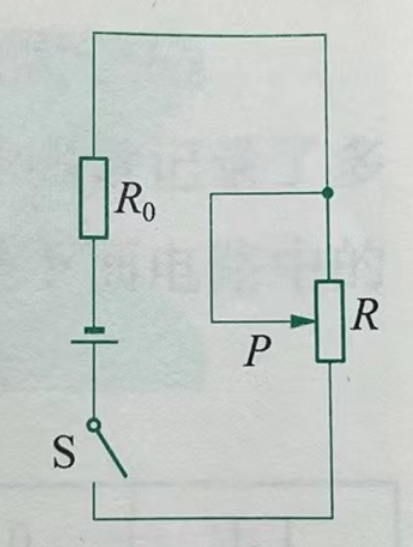
\includegraphics [scale=0.4,trim=0 0 0 0]{./image/physics_circuit4_1.png}
            % \caption{例1图}
            \label{fig:fig_circuit4_1}
        \end{figure}
        \vspace{1.5cm}

        \question[5] 如图所示是某电热器的工作原理图,$R_1, R_2$是发热电阻,虚线框为电热器的金属外壳。它用一个旋转开关可以实现电热器多挡位工作的要求。
        其中旋转开关内有一块绝缘圆盘,在圆盘的左边缘依次有$4$个金属触点,右边缘是一金属板,可绕中心轴转动的开关旋钮两端各有一个金属滑片,
        转动开关旋钮可以将左边缘相邻的两个触点与右边缘的金属板同时连通。如旋到图中位置$S$时,金属滑片将$1$、$2$ 两触点同时与右边缘金属板接通。
        若电源电压为$220V$,则由图可知:
        \begin{subquestions}
            \subquestion 图中$P$、$Q$两个接头中,\underline{\quad\quad\quad\quad}与零线相连;正常情况下,零线和地线的电压为\underline{\quad\quad\quad\quad}$V$。
            \subquestion 为安全起见,需要再电路中安装一个总开关,该开关最好安装在图$A,B,C,D,E$中的\underline{\quad\quad\quad\quad}处。
            \subquestion 如果$R_1=R_2=48.4\Omega$,则电热器在旋钮处于$T$位置时的电功率为\underline{\quad\quad\quad\quad}$W$,当旋钮
            旋到$M$时,通电$1$分钟产生的热量是\underline{\quad\quad\quad\quad}$J$。
        \end{subquestions}
        \begin{figure}[htb]
            \flushright
            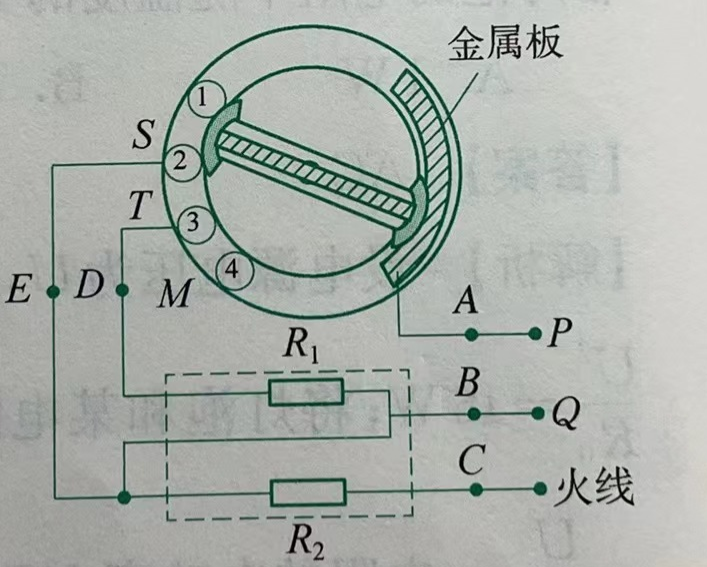
\includegraphics [scale=0.4,trim=0 0 0 0]{./image/physics_circuit4_2.png}
            % \caption{例1图}
            \label{fig:fig_circuit4_2}
        \end{figure}
        \vspace{3.5cm}

        \question[5] 用电阻$13\Omega$的均匀电阻丝制成一个圆环,并把它接到如图所示的电路中。图中导线的$P$端能沿圆环移动,并保持良好接触。
        已知$R_0$为$2\Omega$,电源电压保持$3V$不变。改变$P$的位置,圆环的最大电功率为\underline{\quad\quad\quad\quad}$W$
        \begin{figure}[htb]
            \flushright
            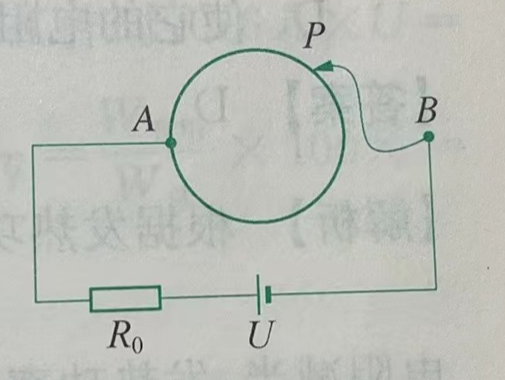
\includegraphics [scale=0.4,trim=0 0 0 0]{./image/physics_circuit4_3.png}
            % \caption{例1图}
            \label{fig:fig_circuit4_3}
        \end{figure}
        \vspace{1.5cm}

        \question[5] 在如图所示的电路中,电源两端电压不变。当只闭合开关$S$、$S_3$。时,电流表的示数$I_1$,电路的总功率是$3W$;
        当开关$S$、$S_1$、$S_2$、$S_3$都闭合时,电流表的示数为$I_2$,电路的总功率是$10.5W$,电阻$R_2$的功率是$4.5W$。求:
        \begin{subquestions}
            \subquestion 电流$I_1$和$I_2$之比。
            \subquestion 电阻$R_1$和$R_3$的比值。
            \subquestion 只闭合开关$S$、$S_2$时,电阻$R_1$的电功率。
        \end{subquestions}
        \begin{figure}[htb]
            \flushright
            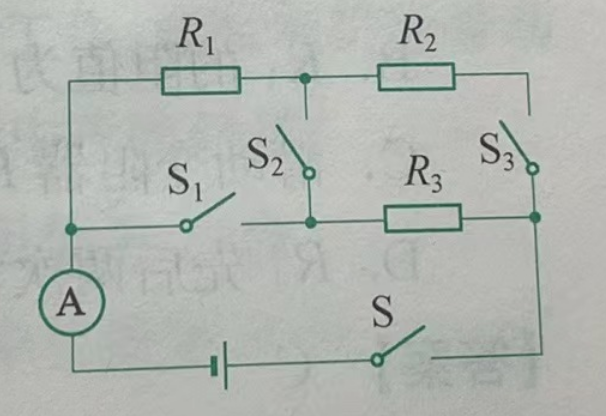
\includegraphics [scale=0.4,trim=0 0 0 0]{./image/physics_circuit4_4.png}
            % \caption{例1图}
            \label{fig:fig_circuit4_4}
        \end{figure}




    \end{questions}





\end{groups}


\label{lastpage}
\end{document}
